\section{Auswertung}
\label{sec:Auswertung}

% % Examples
% \begin{equation}
%   U(t) = a \sin(b t + c) + d
% \end{equation}
%
% \begin{align}
%   a &= \input{build/a.tex} \\
%   b &= \input{build/b.tex} \\
%   c &= \input{build/c.tex} \\
%   d &= \input{build/d.tex} .
% \end{align}
% Die Messdaten und das Ergebnis des Fits sind in Abbildung~\ref{fig:plot} geplottet.
%
% %Tabelle mit Messdaten
% \begin{table}
%   \centering
%   \caption{Messdaten.}
%   \label{tab:data}
%   \sisetup{parse-numbers=false}
%   \begin{tabular}{
% % format 1.3 bedeutet eine Stelle vorm Komma, 3 danach
%     S[table-format=1.3]
%     S[table-format=-1.2]
%     @{${}\pm{}$}
%     S[table-format=1.2]
%     @{\hspace*{3em}\hspace*{\tabcolsep}}
%     S[table-format=1.3]
%     S[table-format=-1.2]
%     @{${}\pm{}$}
%     S[table-format=1.2]
%   }
%     \toprule
%     {$t \:/\: \si{\milli\second}$} & \multicolumn{2}{c}{$U \:/\: \si{\kilo\volt}$\hspace*{3em}} &
%     {$t \:/\: \si{\milli\second}$} & \multicolumn{2}{c}{$U \:/\: \si{\kilo\volt}$} \\
%     \midrule
%     \input{build/table.tex}
%     \bottomrule
%   \end{tabular}
% \end{table}
%
% % Standard Plot
% \begin{figure}
%   \centering
%   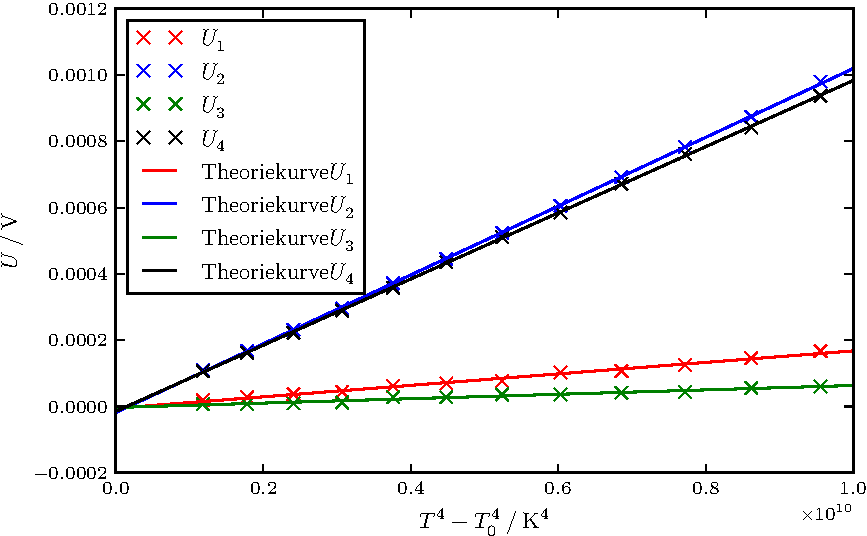
\includegraphics{build/plot.pdf}
%   \caption{Messdaten und Fitergebnis.}
%   \label{fig:plot}
% \end{figure}
%
% 2x2 Plot
% \begin{figure*}
%     \centering
%     \begin{subfigure}[b]{0.475\textwidth}
%         \centering
%         \includegraphics[width=\textwidth]{Abbildungen/Schaltung1.pdf}
%         \caption[]%
%         {{\small Schaltung 1.}}
%         \label{fig:Schaltung1}
%     \end{subfigure}
%     \hfill
%     \begin{subfigure}[b]{0.475\textwidth}
%         \centering
%         \includegraphics[width=\textwidth]{Abbildungen/Schaltung2.pdf}
%         \caption[]%
%         {{\small Schaltung 2.}}
%         \label{fig:Schaltung2}
%     \end{subfigure}
%     \vskip\baselineskip
%     \begin{subfigure}[b]{0.475\textwidth}
%         \centering
%         \includegraphics[width=\textwidth]{Abbildungen/Schaltung4.pdf}    % Zahlen vertauscht ... -.-
%         \caption[]%
%         {{\small Schaltung 3.}}
%         \label{fig:Schaltung3}
%     \end{subfigure}
%     \quad
%     \begin{subfigure}[b]{0.475\textwidth}
%         \centering
%         \includegraphics[width=\textwidth]{Abbildungen/Schaltung3.pdf}
%         \caption[]%
%         {{\small Schaltung 4.}}
%         \label{fig:Schaltung4}
%     \end{subfigure}
%     \caption[]
%     {Ersatzschaltbilder der verschiedenen Teilaufgaben.}
%     \label{fig:Schaltungen}
% \end{figure*}

\subsection{Bestimmung der freien Weglänge}
Zunächst werden die Sättigungsdampfdrücke $p_{\text{sätt}}$ aus Formel \eqref{eqn:8} sowie die mittleren Wegländen der Elektronen aus Formel \eqref{eqn:7} für die verschiedenen Temperaturen, bei denen die Experimente durchgeführt werden, bestimmt.
Die Ergebnisse sind in Tabelle \ref{tab:0} angegeben.
\begin{table}
    \centering
    \caption{Bestimmung der Schallgeschwindigkeit mittels Impuls-Echo-Verfahren.}
    \label{tab:0}
    \sisetup{parse-numbers=false}
    \begin{tabular}{
	S[table-format=3.2]
	S[table-format=2.1]
	S[table-format=4.2]
	}
	\toprule
	{$h_{\text{zylinder}} \:/\: 10^{-3} \si{\metre}$}		& {$\increment t \:/\: 10^{-6} \si{\second} $}		& 
	{$c_\text{Acryl} \:/\: \si{\metre\per\second} $}		\\ 
	\midrule
    61.50  & 44.9 & 2739.42 \\
80.55  & 58.3 & 2763.29 \\
102.10 & 75.0 & 2722.67 \\
120.50 & 87.4 & 2757.44 \\
92.60  & 67.8 & 2731.56 \\
111.85 & 81.1 & 2758.32 \\

    \bottomrule
    \end{tabular}
    \end{table}


\subsection{Integrale Energieverteilung}
Wie in der Durchführung beschrieben wird eine feste Beschleunigungsspannung von $U_b = \SI{11}{\volt}$ gewählt, und der Auffängerstrom gemessen.
Um nun die integrale Energieverteilung beschreiben zu können, weden mehrere Spannungswerte $U_a$ gegen den dazugehörigen Wert
\begin{equation}
  \increment I_a \coloneq I_a(U_a) - I_a(U_a + \increment U_a)
\end{equation}
abgetragen.
Dementsprechend beschreibt dieser Zusammenhang nach der Formel \eqref{eqn:3} die Energieverteilung, da eine hohe Änderung von $I_a$ einer hohen Anzahl von Elektronen entspricht, die ebendiese kinetische Energie besitzen und nun durch die Bremsspannung aufgehalten werden.
Zur Bestimmung der Spannungsdifferenzen werden die Werte
\begin{align*}
  \increment U_{a,1} = \SI{0,394}{\volt} \\
  \increment U_{a,2} = \SI{0.292}{\volt}
\end{align*}
verwendet.
Die Ergebnisse sind in den Tabellen \ref{tab:1} und \ref{tab:2} dargestellt sowie in den Abbildungen \ref{fig:plot1} und \ref{fig:plot2} graphisch dargestellt.
Auf eine Betrachtung der Messfehler wird hier verzichtet, da die Ablesefehler aus dem Diagramm einen größeren Faktor darstellen.

\begin{table}
    \centering
    \caption{Messwerte für die Integrale Energieverteilung bei $T = \SI{26.1}{\celsius}$.}
    \label{tab:1}
    \sisetup{parse-numbers=false}
    \begin{tabular}{
	S[table-format=1.2]
	S[table-format=3.2]
	}
	\toprule
	{$U_a  /  \si{\volt}$}		& {$\increment I_a \:/\: 10^{-9} \si{\ampere}$}		\\ 
	\midrule
    0.00 & 26.68  \\
1.18 & 26.68  \\
2.36 & 26.68  \\
3.55 & 30.02  \\
4.73 & 36.69  \\
5.91 & 46.69  \\
7.09 & 73.37  \\
7.49 & 83.38  \\
7.88 & 153.41 \\
8.27 & 30.02  \\
9.46 & 0.00   \\

    \bottomrule
    \end{tabular}
    \end{table}

\begin{table}
    \centering
    \caption{Messwerte für die Integrale Energieverteilung bei $T = \SI{145.5}{\celsius}$.}
    \label{tab:2}
    \sisetup{parse-numbers=false}
    \begin{tabular}{
	S[table-format=1.2]
	S[table-format=1.2]
	}
	\toprule
	{$U_a  /  \si{\volt}$}		& {$\increment I_a \:/\: 10^{-9} \si{\ampere}$}		\\ 
	\midrule
    0.00 & 0.88 \\
0.58 & 0.80 \\
1.17 & 0.70 \\
1.75 & 0.65 \\
2.34 & 0.53 \\
2.63 & 0.48 \\
2.92 & 0.35 \\
3.21 & 0.25 \\
3.50 & 0.15 \\
3.80 & 0.05 \\
4.38 & 0.00 \\
4.96 & 0.00 \\
5.55 & 0.00 \\
6.13 & 0.00 \\

    \bottomrule
    \end{tabular}
    \end{table}


\begin{figure}[H]
  \centering
  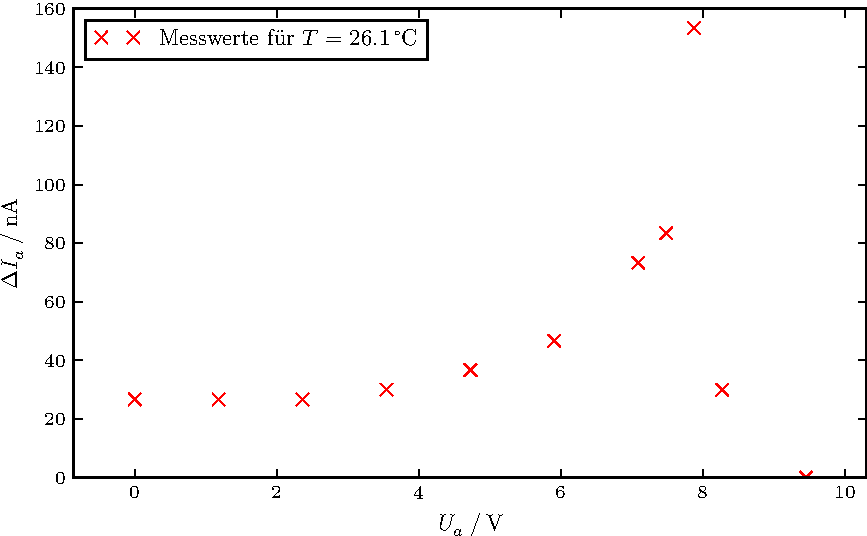
\includegraphics{build/aufgabenteil_a_plot.pdf}
  \caption{Messdaten für die Integrale Energieverteilung.}
  \label{fig:plot1}
\end{figure}

\begin{figure}[H]
  \centering
  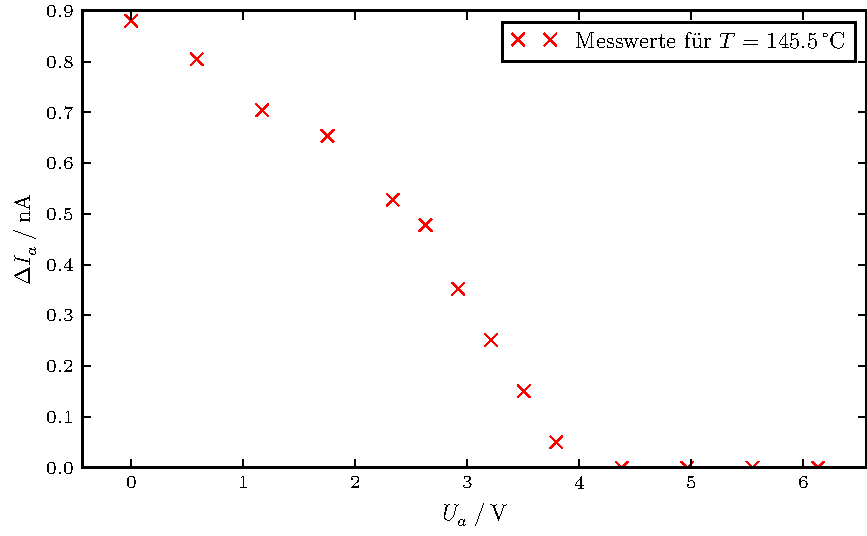
\includegraphics{build/aufgabenteil_a_plot_2.pdf}
  \caption{Messdaten für die Integrale Energieverteilung.}
  \label{fig:plot2}
\end{figure}

Für die erste Messung ist auffällig, dass ein Peak bei ca. $U_{\text{grenz}} = \SI{7.9}{\volt}$ existiert.
Da die Beschleunigungsspannung größer als diese effektive Elektronenenergie nach Durchlaufen des elektrischen Feldes ist, kann man von einem sich hier auswirkenden Kontaktpotential ausgehen.
Dieses beträgt dementsprechend ca. $K = \SI{2.1}{\volt}$.\\
In der zweiten Messung erweist sich eine konkrete Zuordnung eines Peaks als schwieriger.
Dies liegt vermutlich an der Tatsache, dass deutlich mehr inelastische Stöße stattfinden, da die mittlere Weglänge im Vergleich zur Messung bei Zimmertemperatur deutlich geringer ist.
Ein theoretisch zu erwartender bei
\begin{equation}
  U = U_b - K - U_{\text{Hg}}
\end{equation}
ist leicht zu sehen. %hier dann konkret werden wenn U_hg bei Teil b berechnet wurde.

\subsection{Interpretation der Franck-Hertz Kurven}
